% -*- TeX -*-
%
% ----------------------------------------------------------------------
%
%                           Brad T. Aagaard
%                        U.S. Geological Survey
%
% {LicenseText}
%
% ----------------------------------------------------------------------
%

\documentclass[pdftex,cig,slideColor]{pp4slides}
\usepackage{amsmath}
\usepackage{array}
\usepackage{xspace}
\usepackage{multirow}
\usepackage{ulem}

\title{}
\subtitle{}
\author{Brad Aagaard}
\institution{}
\date{June 14, 2008}

% --------------------------------------------------------- DOCUMENT
\begin{document}

\bgadd{\vspace*{7.9in}%
  \begin{center}%
    \includegraphics[height=14mm]{../../logos/cig}\hspace{15mm}
    
\includegraphics[height=14mm]{figs/SCEC_logored}\hspace{15mm}
    
\includegraphics[height=14mm]{figs/nsf_logo}\hspace{15mm}
    
\includegraphics[height=14mm]{figs/NASAlogo}
  \end{center}}

% ------------------------------------------------------------ SLIDE
\foilhead{Overview of Workshop}
  \summary{Draft agenda posted on geodynamics.org}
 
  \vfill
  \begin{center}
    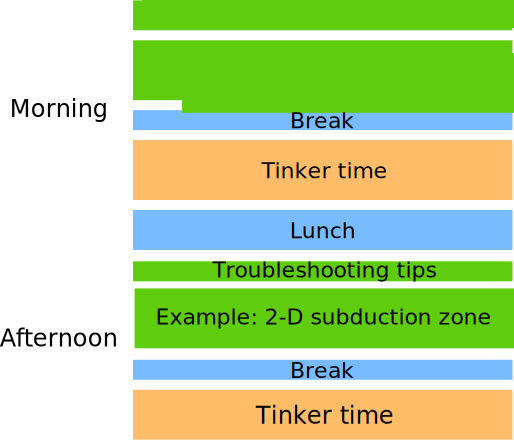
\includegraphics[scale=0.7]{figs/overview}
  \end{center}  

% ------------------------------------------------------------ SLIDE
\foilhead{Overview of Monday}
  \summary{}

  \begin{itemize}
  \item Morning - Overview of tools
    \begin{itemize}
    \item Overview of workflow
    \item Introduction to modeling software
    \end{itemize}
  \item Afternoon - Hands-on/detailed tutorials
    \begin{itemize}
    \item PyLith/CUBIT
    \item GeoFEST
    \item LaGriT
    \item Tinker time
    \end{itemize}
 \end{itemize}

% ------------------------------------------------------------ SLIDE
\foilhead{Overview of Tuesday}
  \summary{}
 
  \begin{itemize}
  \item Morning
    \begin{itemize}
    \item Overview of new features in modeling software
    \item Intermediate meshing tutorials
      \begin{itemize}
      \item CUBIT
      \item LaGriT
      \end{itemize}
    \item Friction, small strains, and plasticity in PyLith
    \end{itemize}
  \item Afternoon
    \begin{itemize}
    \item Extending PyLith tutorial
    \item Tinker time
   \end{itemize}
  \end{itemize}

% ------------------------------------------------------------ SLIDE
\foilhead{\ }
  \summary{}

  \vfill
  \begin{center}
    {\LARGE 9th Crustal Deformation Modeling Workshop}
  \end{center}
  \vfill
 
% ------------------------------------------------------------ SLIDE
\foilhead{Overview of Workshop}
  \summary{Draft agenda posted on geodynamics.org}
 
  \vfill
  \begin{center}
    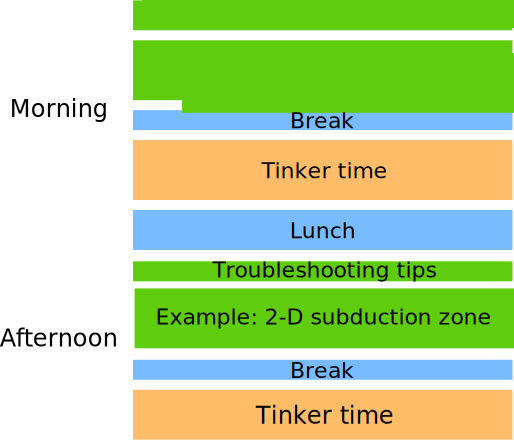
\includegraphics[scale=0.7]{figs/overview}
  \end{center}  

% ------------------------------------------------------------ SLIDE
\foilhead{Participants from Several Communities}

  \vfill
  \begin{center}
    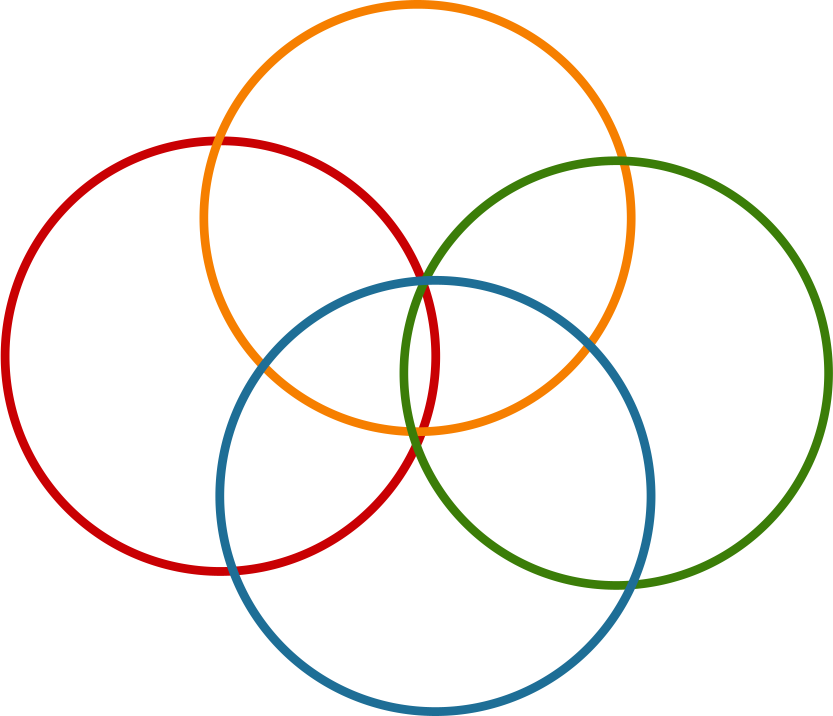
\includegraphics[scale=0.8]{figs/communities}
  \end{center}  

\bgclear
\bgadd{}

% ------------------------------------------------------------ SLIDE
\foilhead{CIG and SCEC News}
  \summary{}
 
  \begin{itemize}
  \item Computational Infrastructure for Geodynamics (CIG)
    \begin{itemize}
    \item Proposal to NSF EAR was funded
    \item Louise Kellogg (UC Davis) is the new Director
    \item New staff being hired this summer
    \item Some previous staff being rehired this summer
  \end{itemize}
  \item Southern California Earthquake Center (SCEC)
    \begin{itemize}
    \item SCEC-4 proposal was submitted in Feb 2010
    \item NSF/USGS site visit to SCEC next week
   \end{itemize}
  \end{itemize}
 
\bgadd{\vspace*{7.9in}%
  \begin{center}%
    \includegraphics[height=14mm]{../../logos/cig}\hspace{15mm}
    
\includegraphics[height=14mm]{figs/SCEC_logored}\hspace{15mm}
    
\includegraphics[height=14mm]{figs/nsf_logo}\hspace{15mm}
    
\includegraphics[height=14mm]{figs/NASAlogo}
  \end{center}}


% ------------------------------------------------------------ SLIDE
\foilhead{Workshop Organizing Committee}
  \summary{}
 
  \begin{itemize}
  \item Brad Aagaard, United States Geological Survey (Chair)
  \item Thorsten Becker, University of Southern California
  \item Andrew Freed, Purdue University
  \item Carl Gable, Los Alamos National Laboratory
  \item Eric Hetland, University of Michigan
  \item Rowena Lohman, Cornell University
  \item Brendan Meade, Harvard University
  \item Mark Simons, California Institute of Technology
  \item Charles Williams, GNS Science
 \end{itemize}

% ------------------------------------------------------------ SLIDE
\foilhead{Community Mission Statement}
  \summary{}
 
  \begin{itemize}
  \item Build tools to understand the response to single earthquakes,
    and make geodetic comparisons, infer rheology, and constrain
    structures
  \item Build tools to simulate fault system interaction, regional
    strain and stress field evolution and produce results that assist
    in the estimation or modeling of fault slip and constrain physics
  \item Develop understanding of transient stress interaction among
    faults
  \item Determine realistic predictions of geologic features (e.g.,
    topography, fault slip)
  \end{itemize}
  
% ------------------------------------------------------------ SLIDE
\foilhead{Workshop Objectives}
  \summary{Make sure everyone's toolbox is filled with useful tools}
 
  \begin{itemize}
  \item Participants will leave the workshop knowing how to do more
    with state-of the-art modeling tools
    \begin{itemize}
    \item Understand the tools themselves
    \item Effective approaches for using them to solve real scientific problems
    \end{itemize}
  \item Define a small number of benchmark problems to 
    \begin{itemize}
    \item Verify codes accurately solve the problems of interest and
      ascertain their strengths and weaknesses
    \item Drive development of new features in codes
    \end{itemize}
  \item Identify computational tools and techniques that will help us
    overcome obstacles in our research
  \end{itemize}
  
% ------------------------------------------------------------ SLIDE
\foilhead{Logistics}
  \summary{}

  \begin{itemize}
  \item Reimbursement forms will be distributed via email
  \item Meals
    \begin{itemize}
    \item Breakfast and lunch provided (Mon-Fri)
    \item Dinner on your own
    \end{itemize}
 \item Posters
    \begin{itemize}
    \item Introductions: Maximum 2 slides as PDF file
    \item Put up your posters at lunch
    \end{itemize}
  \end{itemize}

% ======================================================================
\end{document}


% End of file
